\lstset{ %
  backgroundcolor=\color{white},   % choose the background color; you must add \usepackage{color} or \usepackage{xcolor}
  basicstyle=\footnotesize,             % the size of the fonts that are used for the code
  breakatwhitespace=false,            % sets if automatic breaks should only happen at whitespace
  breaklines=true,                 	   % sets automatic line breaking
  captionpos=b,                    	   % sets the caption-position to bottom
  commentstyle=\color{dkgreen},   % comment style
  deletekeywords={...},            	   % if you want to delete keywords from the given language
  escapeinside={\%*}{*)},             % if you want to add LaTeX within your code
  extendedchars=true,                    % lets you use non-ASCII characters; for 8-bits encodings only, does not work with UTF-8
  frame=single,	                        % adds a frame around the code
  keepspaces=true,                         % keeps spaces in text, useful for keeping indentation of code (possibly needs columns=flexible)
  keywordstyle=\color{blue},          % keyword style
  otherkeywords={*,...},                % if you want to add more keywords to the set
  numbers=left,                               % where to put the line-numbers; possible values are (none, left, right)
  numbersep=5pt,                           % how far the line-numbers are from the code
  numberstyle=\tiny\color{gray},   % the style that is used for the line-numbers
  rulecolor=\color{black},                % if not set, the frame-color may be changed on line-breaks within not-black text (e.g. comments (green here))
  showspaces=false,                       % show spaces everywhere adding particular underscores; it overrides 'showstringspaces'
  showstringspaces=false,              % underline spaces within strings only
  showtabs=false,                           % show tabs within strings adding particular underscores
  stepnumber=1,                             % the step between two line-numbers. If it's 1, each line will be numbered
  stringstyle=\color{mauve},          % string literal style
  tabsize=2,	                                  % sets default tabsize to 2 spaces
  title=\lstname                               % show the filename of files included with \lstinputlisting; also try caption instead of title
}

\chapter{Musiksequenzen mit Hilfe von DL4J erzeugen (unfinished)}
{
Dieses Kapitel befasst sich mit der Umsetzung eines LSTM-Netzwerkes, welches anhand einer gegebenen Beispielmusik Musiksequenzen generiert und dessen Implementierung in DeepLearning4J (DL4J). Als Musikformat wurden MIDI-Dateien gew"ahlt und es wurden zwei Ans"atze zur Verwaltung und Benutzung der Daten verfolgt.

Aufgeteilt ist dieses Kapitel in die Bereiche Eingabe, Netzwerk, Ausgabe und m"ogliche Erweiterungen und Verbesserungen. Die Eingabe umfasst die Themen {\glqq}Was sind MIDI-Dateien?{\grqq}, wie wurden MIDI-Dateien f"ur diese Arbeit eingelesen (inklusive einer Erl"auterung der zwei Implementierungsans"atze) und anschlie{\ss}end in das DL4J DataSet-Format gebracht. Der Abschnitt Netzwerk erl"autert den Aufbau des verwendeten LSTM-Netzwerkes und geht kurz auf die Unterschiede ein, die durch die zwei Ans"atze der Datenverwaltung entstehen. Der Abschnitt Ausgabe geht auf die Bereiche der Ermittlung der Netzwerkausgabe, die Umwandlung der Ausgabe in MIDI-Dateien und die vom Netzwerk erzeugten Ergebnisse ein. Abschlie{\ss}end folgt eine Sammlung von Ideen, wie die Umsetzung erweitert oder verbessert werden k"onnte.


\section{Die Eingabe}

\subsection{Was sind MIDI-Dateien?}
Das Musical Instrument Digital Interface (MIDI) Format wird zum Speichern von Audiodateien benutzt. Im Gegensatz zu anderen Formaten enth"allt eine MIDI-Datei eine Liste von Ereignissen, die zum Beispiel von einer Soundkarte in entsprechende T"one umgewandelt werden k"onnen. 
\begin{quote}{\glqq}Dadurch sind die MIDI-Dateien sehr viel kleiner als digitale Audiodateien, und die Ereignisse und Kl"ange sind editierbar, wodurch die Musik neu arrangiert, editiert und interaktiv Komponiert werden kann.{\grqq} - - - \cite{ITwissen}\end{quote} 
MIDI-Dateien bestehen aus einer Sequenze, die einen oder mehrere Tracks beinhaltet, welchen wiederum Ereignisse zugeordnet sind. Diese Ereignisse k"onnen als Nachrichten ausgelesen werden und besitzen eine MIDI-Zeit, die in Ticks angegeben ist. Abbildung 4.1 zeigt den Aufbau so einer Nachricht, welche aus zwei Teilen, Status und Daten, besteht. Das Statusbyte beginnt immer mit einer 1, gefolgt von drei Bits, die die Art der Nachricht enthalten (in Abbildung 4.1 mit s gekennzeichnet). Die letzten vier Bits geben einen von 16 m"oglichen Kan"alen an (in Abbildung 4.1 mit n gekennzeichnett).
Die Datenbytes beginnen immer mit einer 0 und geben somit Raum f"ur 128  m"ogliche Werte.
\renewcommand{\figurename}{Abb.}
\begin{figure}[htp]
\centering
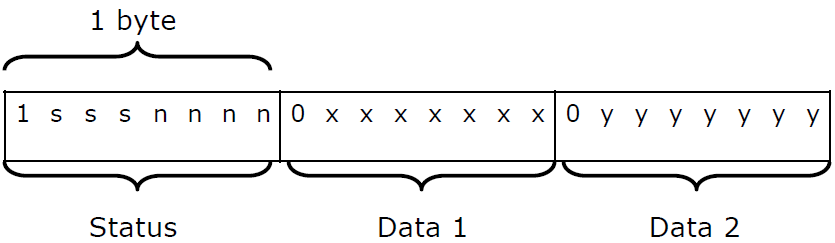
\includegraphics[width=0.60\textwidth]{pictures/MIDI-Message.png}
\caption[MIDI Nachricht]{MIDI Nachricht (Quelle: \cite{MIDIImg})}
\end{figure}

Tabelle \ref{tbl:midiMess} zeigt beispielhaft den Aufbau der Nachrichten {\glqq}Note aus{\grqq} und {\glqq}Note an{\grqq}. Das n im Statusbyte steht f"ur die Kanalnummer, welche Hexadezimal angegeben wird und somit einen Bereich von 0 bis F umfasst. Daten 1 enth"allt eine der 128 m"oglichen Noten und Daten 2 die Geschwindigkeit bzw. die Intensit"at mit der die Note gespielt oder losgelassen wird. Eine {\glqq}Note an{\grqq}-Nachricht mit der Geschwindigkeit 0 ist gleichbedeutend zu {\glqq}Note aus{\grqq}.
(\cite{MIDI})

\begin{table} [h]
\centering
%%\begin{tabular}{|p{0.8cm}|p{3.7cm}|p{8.8cm}|p{8.8cm}|}\hline
\begin{tabular}{|c|c|c|c|}\hline
   \textbf{Nachricht} & \textbf{Status} & \textbf{Daten 1} & \textbf{Daten 2}\\ \hline
   Note aus & 8n & Notennummer & Geschwindigkeit \\ \hline
   Note an & 9n & Notennummer & Geschwindigkeit \\ \hline
 \end{tabular}
\caption{MIDI Nachrichtenformat}
\label{tbl:midiMess} % Verweis im Text mittels \ref{tbl:midiMess}
\end{table}


\subsection{MIDI-Dateien lesen}
Zum Einlesen einer MIDI-Datei wurde eine Java-Klasse geschrieben, die die Tracks einer Sequenze durchl"auft und alle {\glqq}Note an{\grqq} und {\glqq}Note aus{\grqq}-Ereignisse in richtiger Reihenfolge abspeichert. Um die Komplexit"at dieses Projektes am Anfang zu verkleinern, wurde auf die Erfassung der MIDI-Zeit erstmal verzichtet und der Schwerpunkt auf die reine Ereignisabfolge gelegt. Geplant war diese Komponente zu ber"ucksichtigen, sobald das LSTM-Netzwerk in der Lage war eine harmonische Musiksequenze anhand von gelernten Notenfolgen zu erzeugen. Da dieses Ziel aber nicht zufriedenstellend erreicht werden konnte, blieb hierf"ur leider keine Zeit mehr.

F"ur das Abspeichern der Ereignisse wurden die folgenden zwei Ans"atze implementiert:

\subsubsection{Variante 1: Ereignisobjekt}
Die erste Idee der Datenverwaltung war die eines Ereignisobjektes. Da ein MIDI-Ereignis sich aus drei Hauptkomponenten, Note, Geschwindigkeit und Typ (an/aus) zusammensetzt, wurden diese als Variablen gew"ahlt und die Ber"ucksichtung des MIDI-Kanals vorerst ausgelassen. Quellcode \ref{lst:midiEvents} zeigt den Konstruktor f"ur so ein Objekt. In ein solches Objekt werden die Ereignisse einer MIDI-Datei komponentenweise zu Beginn eingelesen. Dadurch erh"allt man drei Listen in der Gr"o{\ss}e des geladenen Musikst"uckes, bzw. der Anzahl der Ereignisse dieses St"uckes.
\lstinputlisting[language=JAVA, firstline=1, lastline=5,  captionpos=b, caption={MidiEvents Konstruktor}, label=lst:midiEvents]
{code_snippets/midiEvents_auszug.java}
Diese Listen enthalten in vermutlich allen F"allen doppelte Werte, da es unwahrscheinlich ist, dass ein Musikst"uck nur aus unterschiedlichen Noten und Geschwindigkeiten besteht. Somit muss noch eine Ermittlung der tats"achlich benutzten Werte erfolgen. F"ur den Ereignistyp ist bekannt, dass er nur zwei Werte annehmen kann. Die Ermittlung der Anzahl der verschiedenen Noten und Geschwindigkeiten wurde wie im Quellcode \ref{lst:matrixValidData} gezeigt umgesetz.
\lstinputlisting[language=JAVA, firstline=20, lastline=30,  captionpos=b, caption={Ereignisobjekt: Listen von g"ultigen Daten}, label=lst:matrixValidData]
{code_snippets/app_auszug.java}
Die Liste der Noten (Codezeilen 1 bis 5) und die Liste der Geschwindigkeiten (Codezeilen 7 bis 11) wurden einmal komplett durchlaufen und mit Hilfe eines LinkedHashSet alle benutzten Werte je einmal erfasst. Anschlie{\ss}end erfolgt eine Abspeicherung der Werte in eine ArrayList. W"urde man diese Reduzierung nicht machen, m"usste man das Netzwerk so auslegen, dass es in der Lage ist den Zusammenhang von 32768 (128*128*2) m"oglichen Ereignissen zulernen.

Nun stehen die Eingangsdaten als Objekt zum Erstellen einer DL4J DataSets zur Verf"ugung und die Gr"o{\ss}e der Netzwerk-Layer kann durch die Anzahl der verschiedenen Ereignisse in der kompromierten Liste bestimmt werden.

\subsubsection{Variante 2: Ereignisschl"ussel}
Da die erste Variante der Implementierung nicht zum Erfolg f"uhrte, musste ein anderer Wege gefunden werden. Der zweite Ansatz verfolgt die Idee einem Ereignis eine eindeutige Zahl (in dieser Arbeit als Schl"ussel bezeichnet) zu zuweisen. Vorgesehen f"ur diesen Schl"ussel ist ein neunstelliger Integer. Dieser setzt sich zusammen aus einer zweistelligen Kanalnummer, einem einstelligen Ereignistyp, einer dreistelligen Notennummer und einer dreistelligen Geschwindigkeit. Tabelle \ref{tbl:eventKey} zeigt die verwendete Kodierung der Ereignisschl"ussel mit einem Beispiel. Das Beispiel beschreibt das Ereignis {\glqq}Note an{\grqq} f"ur die Note A5 (81) mit der Geschwindigkeit 64 auf Kanal 1.

\begin{table} [h]
\centering
%%\begin{tabular}{|p{0.8cm}|p{3.7cm}|p{8.8cm}|p{8.8cm}|}\hline
\begin{tabular}{|c|c|c|c|c|c|}\hline
   & \textbf{Kanalnr.} & \textbf{Ereignistyp} & \textbf{Notennr.} & \textbf{Geschwindigkeit}& \textbf{Schl"ussel}\\ \hline
  \textbf{Stellen} & kk & t & nnn & ggg & kktnnnggg\\ \hline
  \textbf{Beispiel} & 00 & 1 & 081 & 064 & 001081064\\ \hline
 \end{tabular}
\caption{Ereignisschl"ussel}
\label{tbl:eventKey}
\end{table}

Das Speichern der Daten aus einer MIDI-Datei erfolgt in eine ArrayList "uber Integer, wobei die Ereignisse beim Einlesen direkt in die Schl"usselform gebracht werden. Somit erh"allt man eine Liste aller Ereignisse und kann daraus ermitteln aus wie vielen verschiedenen Ereignissen die Musiksequenze besteht. Quellcode \ref{lst:schlusselValidData} zeigt diese Erfassung, wie schon bei der ersten Variante, mit Hilfe eines LinkedHashSet, wobei {\glqq}track{\grqq} die Liste aller Ereignisse ist.
\lstinputlisting[language=JAVA, firstline=9, lastline=13,  captionpos=b, caption={Ereignisschl"ussel: Liste von g"ultigen Daten}, label=lst:schlusselValidData]
{code_snippets/app_auszug.java}
Auch in dieser Variante stehen nun sowohl die Eingangsdaten zum Erstellen eines DL4J DataSets, sowie die Anzahl der verschiedenen Ereignisse zur Verf"ugung, um die Gr"o{\ss}en der Netzwerk-Layer zu bestimmen.


\subsection{DataSets erstellen}
DL4J Netzwerke arbeiten mit dem Datenformat DataSet, welches aus einem Input und einem Label (Output) bestehen. Da das Netzwerk daraufhin trainiert werden soll, dass es bei Eingabe eines Ereignisses das Folgeereignis mit der h"ochsten Wahrscheinlichkeit ausgibt, wird als Label jeweils das folgende Ereignis zugewiesen.

F"ur die Backpropagation Through Time wird von DL4J die Benutzung von 3-dimensionalen INDArrays f"ur Input und Label gefordert. Hierauf wird in der Beschreibung der zwei Varianten noch einmal eingegangen.

Anders als erwartet, war dieser Bereich einer der schwierigsten in der Umsetzung und hat viel Zeit in Anspruch genommen. Die Umwandlung von den Daten in ein Format mit dem das Netzwerk arbeiten kann, stellte ein gro{\ss}es Verst"andnis voraus, welches zu Beginn der Arbeit noch nicht vorhanden war. Dies f"uhrte zu mehreren Implementierungsfehlern und auch die sonst sehr ausf"uhrliche und verst"andliche Dokumentation von \cite{DL4J} konnte hier die Verst"andnisl"ucken nicht f"ullen. Erst die von \cite{DL4J} zur Verf"ugung gestellten Code-Beispiele vermittelten ein erstes Gef"uhl f"ur die richtige Benutzung, reichten aber nicht aus, um bereits jetzt festzustellen, dass die Variante 1 (Ereignisobjekt) wie geplant nicht umsetzbar ist.

\subsubsection{Variante 1: Ereignisobjekt}
Obwohl diese Implementierung zu keinem Ergebnis gekommen ist, soll hier trotzdem weiter darauf eingegangen werden, um auf die begangenen Fehler und gewonnenen Erkenntnisse hinzuweisen.

Quellcode \ref{lst:matrixData} zeigt die komplette Methode, die zum Erstellen eines DataSets geschrieben wurde. Zeile 3 und 4 legen die 3-dimensionalen INDArrays f"ur den Input und die Labels an. Als erster Parameter wird die Anzahl der Mini-Batches angegeben. Mini-Batches k"onnen in DL4J bei gro{\ss}er Datenmenge in externen Dateien sinnvoll sein. Mit ihnen kann man diese Menge in kleinere St"ucke zerlegen und somit in mehreren Schritten dem Netzwerk zuf"uhren. Das hat den Vorteil, dass nicht alle Daten auf einmal geladen werden m"ussen, sondern immer nur kleinere Teile. In dieser Arbeit wurde auf die Unterteilung in Mini-Batches verzichtet und der erste Parameter ist 1, denn alle Daten werden dem Netzwerk zusammen zugef"uhrt.

Der zweite Parameter ist der Platz f"ur den Eingang und wurde als
\begin{center}{\glqq}Anzahl der verschiedenen Noten{\grqq} * {\glqq}Anzahl der verschiedenen Geschwindigkeiten{\grqq} * 2 \end{center}
festgelegt. Dadurch erh"allt man die Anzahl aller m"oglichen Eing"ange.

Der dritte Parameter gibt die L"ange aller Trainingsdaten an und wurde durch die Gr"o{\ss}e einer der Listen aus dem Ereignisobjekt angegeben.
\lstinputlisting[language=JAVA, firstline=2, lastline=23,  captionpos=b, caption={Ereignisobjekt: Trainingsdaten}, label=lst:matrixData]
{code_snippets/LSTMNetwork_auszug.java}
Anschlie{\ss}end wurde eine For-Schleife zum Bef"ullen des Input und der Label benutzt, welche "uber alle Trainingsdaten iteriert. Von Zeile 7 bis Zeile 12 werden den Variablen ihre zu diesem Ereignis (bzw. dem Folgeereignis) zugeh"origen Werte zu gewiesen, mit der Besonderheit, dass das allerletzte Ereignis das erste Ereignis als Nachfolger erh"allt.

In Zeile 13 werden die Inputs in das INDArray eingetragen und in Zeile 14 die Labels. An dieser Stelle befindet sich der Fehler im Gedankengang und der Implementierung. Der zweite Parameter m"usste eindeutig einem Ereignis zu zuordnen sein, was aber durch die Verwendung des Ereignisobjektes nicht m"oglich ist. Durch diese Art der Implementierung werden verschiedene Ereignisse mit demselben Identifikator versehen, was zu einem falschen Datensatz f"uhrt. Schon hier h"atte auffallen m"ussen, dass das nicht funktioniert, was leider durch die Unsicherheiten in der DataSet-Erstellung nicht passierte.

\subsubsection{Variante 2: Ereignisschl"ussel}
Das Bemerken des Fehlers in der Variante 1 f"uhrte schlie{\ss}lich zur Idee des Ereignisschl"ussels. Da hierbei die Ereignisse nicht aus mehreren kombinierbaren Teilen bestehen, war eine eindeutige Identifikation m"oglich.

Quellcode \ref{lst:schlusselData} zeigt die Implementierung der Methode zum Erstellen eines DataSets f"ur Ereignisschl"ussel. In Zeile 3 und 4 werden die 3-dimensionalen INDArrays f"ur den Input und die Labels angelegt. Wie bei der Variante 1 wurde auf die Benutzung von Mini-Batches verzichtet und der erste Parameter ist 1. Der zweite Parameter, die Anzahl aller m"oglichen Eing"ange, ist durch die Gr"o{\ss}e der Liste mit den verschiedenen Ereignissen festgelegt. Der dritte Parameter ist die Anzahl aller Ereignisse der eingelesenen Musik.
\lstinputlisting[language=JAVA, firstline=26, lastline=43,  captionpos=b, caption={Ereignisschl"ussel: Trainingsdaten}, label=lst:schlusselData]
{code_snippets/LSTMNetwork_auszug.java}
Das Bef"ullen erfolgt mit Hilfe einer For-Schleife, die einmal "uber die Ereignisse der eingelesenen Musik iteriert. Auch hier wird dem letzten Ereignis das Erste als Nachfolger zugewiesen. In den Zeilen 9 und 10 erhalten das Input und Label INDArray ihre Werte. Anzumerken ist hier, dass das DataSet lediglich einen Index auf das Ereignis in der Auflistung der verschiedenen Ereignisse erh"allt und nicht der Ereignisschl"ussel "ubergeben wird.



\section{Das Netzwerk (unfinished)}
Das benutzte LSTM-Netzwerk besteht aus einem Eingangs-, einem Ausgangs- und einem HiddenLayer. Die Varianten des Ereignisobjektes und der Ereignisschl"ussel unterscheiden sich in der Gr"o{\ss}e der Layer, wie nachfolgend erl"autert.

\subsubsection{Variante 1: Ereignisobjekt (unfinished) }
Layergr"o{\ss}en
Quellcode \ref{lst:matrixLayer}
\lstinputlisting[language=JAVA, firstline=32, lastline=33,  captionpos=b, caption={Ereignisobjekt: Gr"o{\ss}e der Ein- und Ausgangslayer}, label=lst:matrixLayer]
{code_snippets/app_auszug.java}
...

\subsubsection{Variante 2: Ereignisschl"ussel (unfinished) }
Layergr"o{\ss}en
Quellcode \ref{lst:schlusselLayer}
\lstinputlisting[language=JAVA, firstline=15, lastline=16,  captionpos=b, caption={Ereignisschl"ussel: Gr"o{\ss}e der Ein- und Ausgangslayer}, label=lst:schlusselLayer]
{code_snippets/app_auszug.java}
...
Version 1: Yiruma track2 = 1040 events, 36 in/output M"oglichkeiten, hidden = in*2 -> zu wenig varianz, lernt eine Note zu spielen
Version 1: F"ur Elise track2 = 1254 events, 417 in/output M"oglichkeiten, hidden = in*2 (hidden = in) -> netz lernt nicht
Version 1: Bumblebee track1 = 2620 events, 1053 in/output M"oglichkeiten, hidden = in*2 (hidden = in) -> out of memory, can not allocate




\section{Die Ausgabe (unfinished)}
\subsection{Auswerten der Netzwerkausgabe (unfinished)}
Zum Erzeugen einer Ausgabe wird dem Netzwerk ein Ereignis als Starteingabe gegeben, woraufhin das Netz ein Folgeereignis ausgibt. Diese Ausgabe wird dem Netzwerk wieder als Eingabe zugef"uhrt und dieser Vorgang wird wiederholt bis die gew"unscht Gr"o{\ss}e der zu erzeugenden Musiksequenz erreicht ist.

Die Auswertung der Netzwerkausgabe erfolgt durch die Ermittlung des Ausganges mit dem h"ochsten Wert.

\subsubsection{Variante 1: Ereignisobjekt (unfinished)}
...Problem erkannt
...Quellcode \ref{lst:matrixOutput}
\lstinputlisting[language=JAVA, firstline=48, lastline=63,  captionpos=b, caption={Ereignisobjekt: Netzausgabe}, label=lst:matrixOutput]
{code_snippets/LSTMNetwork_auszug.java}

\subsubsection{Variante 2: Ereignisschl"ussel (unfinished)}
...
...Quellcode \ref{lst:schlusselOutput}
\lstinputlisting[language=JAVA, firstline=66, lastline=81,  captionpos=b, caption={Ereignisschl"ussel: Netzausgabe}, label=lst:schlusselOutput]
{code_snippets/LSTMNetwork_auszug.java}


\subsection{MIDI Files schreiben (unfinished)}
...

\subsection{Ergebnisse (unfinished)}
- did not have the time nor computational power to experiment further with this
- nur Variante 2, da Variante 1 fehlerhaft ist

\renewcommand{\figurename}{Abb.}
\begin{figure}[htp]
%%\begin{floatingfigure}[r]{textwidth}
\centering
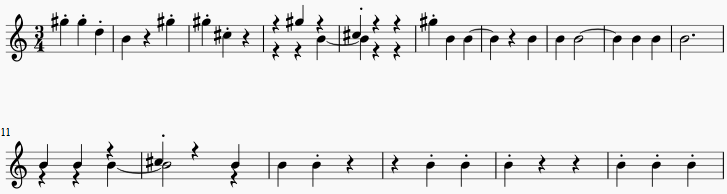
\includegraphics[width=1\textwidth]{pictures/sampleMidi1.png}
\caption[Beispielausgabe 1]{Beispielausgabe 1}
%%\end{floatingfigure} 
\end{figure}

\renewcommand{\figurename}{Abb.}
\begin{figure}[htp]
%%\begin{floatingfigure}[r]{textwidth}
\centering
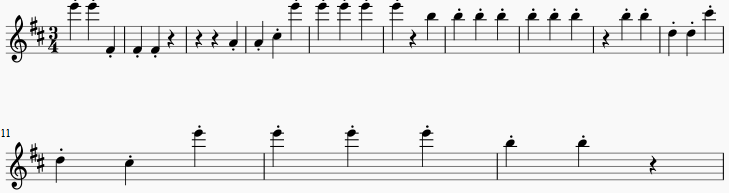
\includegraphics[width=1\textwidth]{pictures/sampleMidi2.png}
\caption[Beispielausgabe 2]{Beispielausgabe 2}
%%\end{floatingfigure} 
\end{figure}

\section{M"ogliche Erweiterungen und Verbesserungen (unfinished)}
- DataSetIterator()
} %% Ende Chapter{Musiksequenzen mit Hilfe von DL4J erzeugen}